\documentclass{article}

% content/resources/templates/preamble.tex
\usepackage[margin=0.6in]{geometry}
\author{Milav Dabgar}
\usepackage{amsmath,amssymb,amsthm}
\usepackage{booktabs}
\usepackage{multirow}
\usepackage{xcolor}
\usepackage{tcolorbox}
\tcbuselibrary{breakable,skins}
\usepackage[colorlinks=true,linkcolor=blue]{hyperref}
\usepackage{titlesec}
\usepackage{enumitem}
\usepackage{tikz}
\usepackage{pgfplots}
\usepackage{circuitikz}
\usepackage[version=4]{mhchem}
\usepackage{longtable}
\usepackage{array}
\usepackage{float}
\usepackage{caption}
\usepackage{listings}

\lstset{
  basicstyle=\small\ttfamily,
  breaklines=true,
  breakatwhitespace=false,
  postbreak=\mbox{\textcolor{red}{$\hookrightarrow$}\space},
  float=false,
  numbers=left,
  numberstyle=\tiny\color{gray},
  numbersep=10pt,
  xleftmargin=2em,
  keywordstyle=\color{blue},
  commentstyle=\color{green!60!black},
  stringstyle=\color{purple},
  backgroundcolor=\color{gray!5},
  showstringspaces=false,
  tabsize=2,
  captionpos=b,
  keepspaces=true,
  columns=flexible
}

\pgfplotsset{compat=1.18}
\usetikzlibrary{shapes,arrows,positioning,calc,patterns,decorations.pathmorphing,decorations.markings,arrows.meta}

% Color scheme
\definecolor{headcolor}{RGB}{0,102,204}
\definecolor{keycolor}{RGB}{220,20,60}
\definecolor{solutioncolor}{RGB}{34,139,34}
\definecolor{mnemoniccolor}{RGB}{148,0,211}
\definecolor{codecolor}{RGB}{0,0,100}

% Spacing
\setlength{\parskip}{3pt}
\setlist[itemize]{nosep}
\setlist[enumerate]{nosep}

% Title formatting
\titleformat{\section}{\Large\bfseries\color{headcolor}}{\thesection}{1em}{}
\titleformat{\subsection}{\large\bfseries\color{headcolor}}{\thesubsection}{1em}{}

% Pandoc tightlist compatibility
\providecommand{\tightlist}{%
  \setlength{\itemsep}{0pt}\setlength{\parskip}{0pt}}

% Pandoc longtable compatibility
\newcounter{none}
\def\thenone{}


% content/resources/templates/english-boxes.tex

% Custom environments
\newtcolorbox{solutionbox}{
 breakable,
 enhanced,
 colback=solutioncolor!5!white,
 colframe=solutioncolor!75!black,
 fonttitle=\bfseries,
 title=Solution
}

\newtcolorbox{solutionboxnobreak}{
 colback=solutioncolor!5!white,
 colframe=solutioncolor!75!black,
 fonttitle=\bfseries,
 title=Solution
}

\newtcolorbox{keyformula}{
 breakable,
 enhanced,
 colback=keycolor!5!white,
 colframe=keycolor!75!black,
 fonttitle=\bfseries,
 title=Key Formula
}

\newtcolorbox{mnemonicboxenv}{
 breakable,
 enhanced,
 colback=mnemoniccolor!5!white,
 colframe=mnemoniccolor!75!black,
 fonttitle=\bfseries,
 title=Mnemonic
}

\newcommand{\mnemonicbox}[1]{%
  \begin{mnemonicboxenv}
    #1
  \end{mnemonicboxenv}
}


% Custom commands for GTU solutions
% This file defines semantic commands for consistent formatting

% Question command with automatic formatting
\newcommand{\question}[2]{%
  \section*{Question #1}%
  \textbf{#2}%
}

% OR question variant
\newcommand{\questionor}[2]{%
  \section*{Question #1 OR}%
  \textbf{#2}%
}

% Proper table environment with caption
\newenvironment{answertable}[1]{%
  \begin{table}[htbp]
  \centering
  \caption{#1}
}{%
  \end{table}
}

% Proper figure environment for diagrams
\newenvironment{answerdiagram}[1]{%
  \begin{figure}[htbp]
  \centering
  \caption{#1}
}{%
  \end{figure}
}

% Semantic markup for key terms
\newcommand{\keyword}[1]{\textbf{#1}}
\newcommand{\code}[1]{\texttt{#1}}
\newcommand{\classname}[1]{\texttt{#1}}
\newcommand{\methodname}[1]{\texttt{#1}}

% Proper quotation marks
\newcommand{\mnemonic}[1]{``#1''}


\title{Introduction To IT Systems (4311602) - Summer 2024 Solution}
\date{June 14, 2024}

\begin{document}
\maketitle

\questionmarks{1(a)}{3}{Define Following Term: 1. Data 2. Information 3. Knowledge}

\begin{solutionbox}
\textbf{Answer:}

\begin{answertable}{Data, Information, and Knowledge Definitions}
\begin{tabulary}{\linewidth}{|L|L|}
\hline
\textbf{Term} & \textbf{Definition} \\
\hline
\keyword{Data} & Raw facts and figures without meaning or context \\
\hline
\keyword{Information} & Processed data that has meaning and is useful \\
\hline
\keyword{Knowledge} & Information combined with experience and understanding \\
\hline
\end{tabulary}
\end{answertable}

\begin{itemize}
    \item \textbf{Data}: Basic building blocks without interpretation
    \item \textbf{Information}: Data processed to provide meaningful context
    \item \textbf{Knowledge}: Information enhanced with human insight and wisdom
\end{itemize}

\begin{mnemonicbox}
\mnemonic{DIK - Data Is Knowledge's foundation}
\end{mnemonicbox}
\end{solutionbox}

\questionmarks{1(b)}{4}{Explain Primary Memory in brief.}

\begin{solutionbox}
\textbf{Answer:}

\begin{answertable}{Primary Memory Characteristics}
\begin{tabulary}{\linewidth}{|L|L|}
\hline
\textbf{Aspect} & \textbf{Description} \\
\hline
\textbf{Definition} & Main memory that directly communicates with CPU \\
\hline
\textbf{Access Speed} & Very fast access time \\
\hline
\textbf{Volatility} & Volatile (loses data when power off) \\
\hline
\textbf{Examples} & RAM, Cache memory \\
\hline
\end{tabulary}
\end{answertable}

\begin{itemize}
    \item \textbf{RAM (Random Access Memory)}: Main working memory for current programs
    \item \textbf{Cache Memory}: Ultra-fast memory between CPU and RAM
    \item \textbf{Volatile Nature}: Data disappears when computer shuts down
    \item \textbf{Direct CPU Access}: CPU can directly read/write data
\end{itemize}

\begin{mnemonicbox}
\mnemonic{Primary is Fast but Forgetful}
\end{mnemonicbox}
\end{solutionbox}

\questionmarks{1(c)}{7}{Explain types of real time OS with example.}

\begin{solutionbox}
\textbf{Answer:}

\begin{answertable}{Real-Time Operating System Types}
\begin{tabulary}{\linewidth}{|L|L|L|L|}
\hline
\textbf{Type} & \textbf{Response Time} & \textbf{Examples} & \textbf{Use Cases} \\
\hline
\keyword{Hard Real-Time} & Guaranteed deadline & QNX, VxWorks & Medical devices, Aircraft \\
\hline
\keyword{Soft Real-Time} & Best effort timing & Windows RT, Linux RT & Multimedia, Gaming \\
\hline
\keyword{Firm Real-Time} & Occasional deadline miss & Embedded Linux & Industrial control \\
\hline
\end{tabulary}
\end{answertable}

\begin{answerdiagram}{Real-Time OS Types}
\begin{tikzpicture}[gtu tree]
    \node [gtu root] {Real-Time OS}
        child { node [gtu child] {Hard Real-Time} 
            child { node [gtu block, fill=orange!10] {Critical Systems} }
        }
        child { node [gtu child] {Soft Real-Time} 
            child { node [gtu block, fill=orange!10] {Multimedia Apps} }
        }
        child { node [gtu child] {Firm Real-Time} 
            child { node [gtu block, fill=orange!10] {Industrial Control} }
        };
\end{tikzpicture}
\end{answerdiagram}

\begin{itemize}
    \item \textbf{Hard Real-Time}: Missing deadline causes system failure
    \item \textbf{Soft Real-Time}: Delayed response reduces performance but system continues
    \item \textbf{Deterministic Response}: Predictable timing behavior is essential
\end{itemize}

\begin{mnemonicbox}
\mnemonic{HSF - Hard, Soft, Firm timing requirements}
\end{mnemonicbox}
\end{solutionbox}

\questionmarks{1(c OR)}{7}{Describe Linux architecture and discuss the mode of the operation of Linux}

\begin{solutionbox}
\textbf{Answer:}

\begin{answerdiagram}{Linux Architecture}
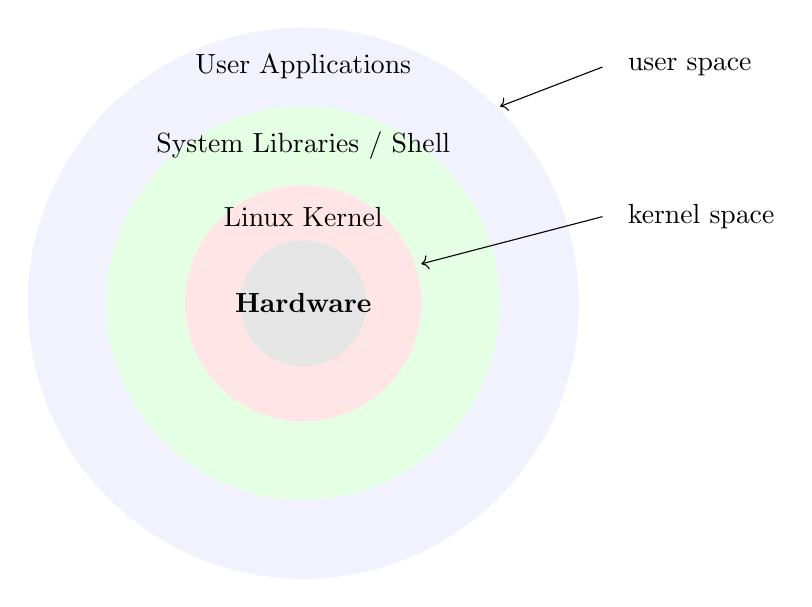
\begin{tikzpicture}[node distance=1.5cm, auto]
    % Concentric circles approach for architecture
    \fill[fill=blue!5] (0,0) circle (3.5cm);
    \fill[fill=green!10] (0,0) circle (2.5cm);
    \fill[fill=red!10] (0,0) circle (1.5cm);
    \fill[fill=gray!20] (0,0) circle (0.8cm);

    \node at (0,0) {\textbf{Hardware}};
    \node at (0, 1.1) {Linux Kernel};
    \node at (0, 2.0) {System Libraries / Shell};
    \node at (0, 3.0) {User Applications};
    
    % Legend or annotations
    \node[anchor=west] at (4, 3) {user space};
    \node[anchor=west] at (4, 1.1) {kernel space};
    \draw[->] (3.8, 3) -- (2.5, 2.5);
    \draw[->] (3.8, 1.1) -- (1.5, 0.5);
\end{tikzpicture}
\end{answerdiagram}

\begin{answertable}{Linux Operation Modes}
\begin{tabulary}{\linewidth}{|L|L|L|L|}
\hline
\textbf{Mode} & \textbf{Description} & \textbf{Access Level} & \textbf{Examples} \\
\hline
\keyword{User Mode} & Restricted access & Limited privileges & Applications, user programs \\
\hline
\keyword{Kernel Mode} & Full system access & Complete control & Device drivers, OS functions \\
\hline
\end{tabulary}
\end{answertable}

\begin{itemize}
    \item \textbf{Layered Architecture}: Clear separation between user and system components
    \item \textbf{Mode Switching}: CPU switches between user and kernel modes
    \item \textbf{System Calls}: Interface for user programs to access kernel services
    \item \textbf{Security}: User mode prevents direct hardware access
\end{itemize}

\begin{mnemonicbox}
\mnemonic{LUSK - Linux Uses Safe Kernel protection}
\end{mnemonicbox}
\end{solutionbox}

\questionmarks{2(a)}{3}{Describe XOR gate with its truth table.}

\begin{solutionbox}
\textbf{Answer:}

\begin{answerdiagram}{XOR Gate Symbol}
\begin{tikzpicture}
    \node[xor gate US, draw, logic gate inputs=nn] (xor) {};
    \draw (xor.input 1) -- ++(-0.5,0) node[left] {A};
    \draw (xor.input 2) -- ++(-0.5,0) node[left] {B};
    \draw (xor.output) -- ++(0.5,0) node[right] {Output ($A \oplus B$)};
\end{tikzpicture}
\end{answerdiagram}

\begin{answertable}{Truth Table}
\begin{tabulary}{\linewidth}{|C|C|C|}
\hline
\textbf{A} & \textbf{B} & \textbf{Output (A $\oplus$ B)} \\
\hline
0 & 0 & 0 \\
\hline
0 & 1 & 1 \\
\hline
1 & 0 & 1 \\
\hline
1 & 1 & 0 \\
\hline
\end{tabulary}
\end{answertable}

\begin{itemize}
    \item \textbf{Exclusive OR}: Output is 1 when inputs are different
    \item \textbf{Logic Function}: $A \oplus B = A'B + AB'$
    \item \textbf{Applications}: Half adder, parity checker, encryption
\end{itemize}

\begin{mnemonicbox}
\mnemonic{XOR - eXclusive OR gives 1 for different inputs}
\end{mnemonicbox}
\end{solutionbox}

\questionmarks{2(b)}{4}{Solve following. i) (4C6)16 = (\_)2 = (\_)10 ii) (186)10 = (\_)8 = (\_)2}

\begin{solutionbox}
\textbf{Answer:}

\begin{answertable}{Solution Summary}
\begin{tabulary}{\linewidth}{|L|L|L|}
\hline
\textbf{Conversion} & \textbf{Step} & \textbf{Result} \\
\hline
\textbf{(4C6)$_{16}$} & Hex to Binary & \textbf{10011000110$_2$} \\
\hline
 & Binary to Decimal & \textbf{1222$_{10}$} \\
\hline
\textbf{(186)$_{10}$} & Decimal to Octal & \textbf{272$_8$} \\
\hline
 & Decimal to Binary & \textbf{10111010$_2$} \\
\hline
\end{tabulary}
\end{answertable}

\textbf{Detailed Solutions:}

i) \textbf{(4C6)$_{16}$ = (10011000110)$_2$ = (1222)$_{10}$}
\begin{itemize}
    \item $4 = 0100, C = 1100, 6 = 0110$
    \item Combined: $010011000110 = 10011000110_2$
    \item Decimal: $1 \times 2^{10} + 0 \times 2^9 + 0 \times 2^8 + 1 \times 2^7 + 1 \times 2^6 + 0 \times 2^5 + 0 \times 2^4 + 0 \times 2^3 + 1 \times 2^2 + 1 \times 2^1 + 0 \times 2^0 = 1222_{10}$
\end{itemize}

ii) \textbf{(186)$_{10}$ = (272)$_8$ = (10111010)$_2$}
\begin{itemize}
    \item Octal: $186 \div 8 = 23 \text{ rem } 2, 23 \div 8 = 2 \text{ rem } 7, 2 \div 8 = 0 \text{ rem } 2 \rightarrow 272_8$
    \item Binary: $186 = 128 + 32 + 16 + 8 + 2 = 10111010_2$
\end{itemize}

\begin{mnemonicbox}
\mnemonic{HDB - Hex, Decimal, Binary conversions}
\end{mnemonicbox}
\end{solutionbox}

\questionmarks{2(c)}{7}{Illustrate following OS: i) Network Operating System ii) Mobile Operating System}

\begin{solutionbox}
\textbf{Answer:}

\begin{answertable}{Operating System Comparison}
\begin{tabulary}{\linewidth}{|L|L|L|}
\hline
\textbf{Feature} & \textbf{Network OS} & \textbf{Mobile OS} \\
\hline
\textbf{Purpose} & Manage network resources & Mobile device management \\
\hline
\textbf{Examples} & Windows Server, Linux Server & Android, iOS, Windows Mobile \\
\hline
\textbf{Key Features} & File sharing, printer sharing & Touch interface, battery management \\
\hline
\textbf{Users} & Multiple simultaneous users & Single user typically \\
\hline
\end{tabulary}
\end{answertable}

\begin{answerdiagram}{OS Types Overview}
\begin{tikzpicture}[gtu tree]
    \node [gtu root] {Operating Systems}
        child { node [gtu child] {Network OS} 
            child { node [gtu block, fill=blue!5] {File Server} }
            child { node [gtu block, fill=blue!5] {Print Server} }
            child { node [gtu block, fill=blue!5] {App Server} }
        }
        child { node [gtu child] {Mobile OS} 
            child { node [gtu block, fill=green!5] {Touch UI} }
            child { node [gtu block, fill=green!5] {App Store} }
            child { node [gtu block, fill=green!5] {Battery Mgmt} }
        };
\end{tikzpicture}
\end{answerdiagram}

\textbf{i) Network Operating System:}
\begin{itemize}
    \item \textbf{Multi-user Support}: Handles multiple concurrent users
    \item \textbf{Resource Sharing}: Files, printers, applications shared across network
    \item \textbf{Security Management}: User authentication and access control
\end{itemize}

\textbf{ii) Mobile Operating System:}
\begin{itemize}
    \item \textbf{Touch-Optimized}: Designed for finger-based interaction
    \item \textbf{Power Management}: Efficient battery usage
    \item \textbf{App Ecosystem}: Centralized app distribution and management
\end{itemize}

\begin{mnemonicbox}
\mnemonic{NOS for Networks, MOS for Mobility}
\end{mnemonicbox}
\end{solutionbox}

\questionmarks{2(a OR)}{3}{Draw Logic circuit of OR gate and NOT gate using only NAND gate.}

\begin{solutionbox}
\textbf{Answer:}

\begin{answerdiagram}{OR Gate using NAND}
\begin{tikzpicture}
    % OR using NAND: (A'B')' = A+B
    \node[nand gate US, draw, logic gate inputs=nn] (n1) at (0,1) {};
    \draw (n1.input 1) -- ++(-0.5,0) node[left] {A}; 
    \draw (n1.input 2) -- ++(-0.5,0) node[left] {A};
    \draw (n1.input 1) -- (n1.input 2);
    
    \node[nand gate US, draw, logic gate inputs=nn] (n2) at (0,-1) {};
    \draw (n2.input 1) -- ++(-0.5,0) node[left] {B};
    \draw (n2.input 2) -- ++(-0.5,0) node[left] {B};
    \draw (n2.input 1) -- (n2.input 2);
    
    \node[nand gate US, draw, logic gate inputs=nn] (n3) at (3,0) {};
    \draw (n1.output) -- (n3.input 1);
    \draw (n2.output) -- (n3.input 2);
    
    \draw (n3.output) -- ++(0.5,0) node[right] {A+B};
\end{tikzpicture}
\end{answerdiagram}

\begin{answerdiagram}{NOT Gate using NAND}
\begin{tikzpicture}
    \node[nand gate US, draw, logic gate inputs=nn] (n1) {};
    \draw (n1.input 1) -- ++(-0.5,0) coordinate (in);
    \draw (n1.input 2) -- ++(-0.5,0);
    \draw (in) -- ++(-0.2,0) node[left] {A};
    \draw (in) ++(0,-0.13) -- (in |- n1.input 2);
    \draw (n1.output) -- ++(0.5,0) node[right] {A'};
\end{tikzpicture}
\end{answerdiagram}

\begin{answertable}{Truth Verification Table}
\begin{tabulary}{\linewidth}{|C|C|C|C|C|}
\hline
\textbf{A} & \textbf{B} & \textbf{A'} & \textbf{B'} & \textbf{(A'$\cdot$B')' = A+B} \\
\hline
0 & 0 & 1 & 1 & 0 \\
\hline
0 & 1 & 1 & 0 & 1 \\
\hline
1 & 0 & 0 & 1 & 1 \\
\hline
1 & 1 & 0 & 0 & 1 \\
\hline
\end{tabulary}
\end{answertable}

\begin{itemize}
    \item \textbf{NAND Universal}: Can implement any logic function
    \item \textbf{De Morgan's Law}: $(A' \cdot B')' = A+B$
\end{itemize}

\begin{mnemonicbox}
\mnemonic{NAND is Universal - can make all gates}
\end{mnemonicbox}
\end{solutionbox}

\questionmarks{2(b OR)}{4}{i) Convert Binary number into Decimal number: (i) 11101 (ii) 10011 ii) Convert decimal number into binary number: (i) 19 (ii) 64}

\begin{solutionbox}
\textbf{Answer:}

\begin{answertable}{Conversion Table}
\begin{tabulary}{\linewidth}{|L|L|L|L|}
\hline
\textbf{Type} & \textbf{Number} & \textbf{Process} & \textbf{Result} \\
\hline
\textbf{Binary to Decimal} & $11101_2$ & $1 \times 2^4+1 \times 2^3+1 \times 2^2+0 \times 2^1+1 \times 2^0$ & \textbf{29$_{10}$} \\
\hline
 & $10011_2$ & $1 \times 2^4+0 \times 2^3+0 \times 2^2+1 \times 2^1+1 \times 2^0$ & \textbf{19$_{10}$} \\
\hline
\textbf{Decimal to Binary} & $19_{10}$ & Division by 2 method & \textbf{10011$_2$} \\
\hline
 & $64_{10}$ & Division by 2 method & \textbf{1000000$_2$} \\
\hline
\end{tabulary}
\end{answertable}

\textbf{Detailed Solutions:}

\textbf{i) Binary to Decimal:}
\begin{itemize}
    \item $11101_2 = 16 + 8 + 4 + 0 + 1 = 29_{10}$
    \item $10011_2 = 16 + 0 + 0 + 2 + 1 = 19_{10}$
\end{itemize}

\textbf{ii) Decimal to Binary:}
\begin{itemize}
    \item $19 \div 2 = 9 \text{ rem } 1, 9 \div 2 = 4 \text{ rem } 1, 4 \div 2 = 2 \text{ rem } 0, 2 \div 2 = 1 \text{ rem } 0, 1 \div 2 = 0 \text{ rem } 1 \rightarrow 10011_2$
    \item $64 \div 2 = 32 \text{ rem } 0... \rightarrow 1000000_2$
\end{itemize}

\begin{mnemonicbox}
\mnemonic{Powers of 2 for Binary to Decimal}
\end{mnemonicbox}
\end{solutionbox}

\questionmarks{2(c OR)}{7}{Explain Open-source software and Proprietary software. Give at least five examples of both the types of software.}

\begin{solutionbox}
\textbf{Answer:}

\begin{answertable}{Software Type Comparison}
\begin{tabulary}{\linewidth}{|L|L|L|}
\hline
\textbf{Aspect} & \textbf{Open-Source} & \textbf{Proprietary} \\
\hline
\textbf{Source Code} & Freely available & Closed/Hidden \\
\hline
\textbf{Cost} & Usually free & Commercial license \\
\hline
\textbf{Modification} & Allowed & Restricted \\
\hline
\textbf{Support} & Community-based & Vendor support \\
\hline
\end{tabulary}
\end{answertable}

\begin{answertable}{Software Examples}
\begin{tabulary}{\linewidth}{|L|L|}
\hline
\textbf{Open-Source} & \textbf{Proprietary} \\
\hline
Linux & Microsoft Windows \\
\hline
LibreOffice & Microsoft Office \\
\hline
Firefox & Internet Explorer \\
\hline
GIMP & Adobe Photoshop \\
\hline
MySQL & Oracle Database \\
\hline
\end{tabulary}
\end{answertable}

\begin{answerdiagram}{Software Distribution}
\begin{tikzpicture}
    \pie[text=legend]{40/Open-Source, 60/Proprietary}
\end{tikzpicture}
\end{answerdiagram}

\begin{itemize}
    \item \textbf{Open-Source Characteristics}: Freedom to modify, Community development, Transparency
    \item \textbf{Proprietary Characteristics}: Commercial model, Professional support, Quality assurance
\end{itemize}

\begin{mnemonicbox}
\mnemonic{FOSS is Free, Open, Shared, Supported by community}
\end{mnemonicbox}
\end{solutionbox}

\questionmarks{3(a)}{3}{Define 1. Modulation 2. Multiplexing}

\begin{solutionbox}
\textbf{Answer:}

\begin{answertable}{Definition Table}
\begin{tabulary}{\linewidth}{|L|L|L|}
\hline
\textbf{Term} & \textbf{Definition} & \textbf{Purpose} \\
\hline
\keyword{Modulation} & Process of varying carrier signal properties & Enable long-distance transmission \\
\hline
\keyword{Multiplexing} & Combining multiple signals for transmission & Efficient channel utilization \\
\hline
\end{tabulary}
\end{answertable}

\begin{itemize}
    \item \textbf{Modulation}: Changes amplitude, frequency, or phase of carrier wave
    \item \textbf{Multiplexing}: Allows multiple users to share same communication medium
    \item \textbf{Signal Processing}: Both techniques improve communication efficiency
\end{itemize}

\begin{mnemonicbox}
\mnemonic{MM - Modulation Modifies, Multiplexing Merges}
\end{mnemonicbox}
\end{solutionbox}

\questionmarks{3(b)}{4}{Explain star topology.}

\begin{solutionbox}
\textbf{Answer:}

\begin{answerdiagram}{Star Topology}
\begin{tikzpicture}[node distance=2.5cm]
    \node[gtu block] (hub) {Hub/Switch};
    \node[gtu child, above=of hub] (pc1) {PC1};
    \node[gtu child, right=of hub] (pc2) {PC2};
    \node[gtu child, below=of hub] (pc3) {PC3};
    \node[gtu child, left=of hub] (pc4) {PC4};
    
    \draw[gtu arrow] (hub) -- (pc1);
    \draw[gtu arrow] (hub) -- (pc2);
    \draw[gtu arrow] (hub) -- (pc3);
    \draw[gtu arrow] (hub) -- (pc4);
\end{tikzpicture}
\end{answerdiagram}

\begin{answertable}{Star Topology Features}
\begin{tabulary}{\linewidth}{|L|L|}
\hline
\textbf{Feature} & \textbf{Description} \\
\hline
\textbf{Central Device} & Hub/Switch connects all nodes \\
\hline
\textbf{Fault Tolerance} & Single node failure doesn't affect others \\
\hline
\textbf{Performance} & Dedicated bandwidth per connection \\
\hline
\textbf{Scalability} & Easy to add/remove nodes \\
\hline
\end{tabulary}
\end{answertable}

\begin{itemize}
    \item \textbf{Central Hub}: All communication passes through central device
    \item \textbf{Easy Troubleshooting}: Problems isolated to individual connections
    \item \textbf{Higher Cost}: Requires more cable than bus topology
    \item \textbf{Single Point of Failure}: Hub failure affects entire network
\end{itemize}

\begin{mnemonicbox}
\mnemonic{STAR - Single point, Troubleshooting easy, All through hub, Reliable}
\end{mnemonicbox}
\end{solutionbox}

\questionmarks{3(c)}{7}{Prepare a short note on Time Division Multiplexing (TDM)}

\begin{solutionbox}
\textbf{Answer:}

\begin{answerdiagram}{Time Division Multiplexing}
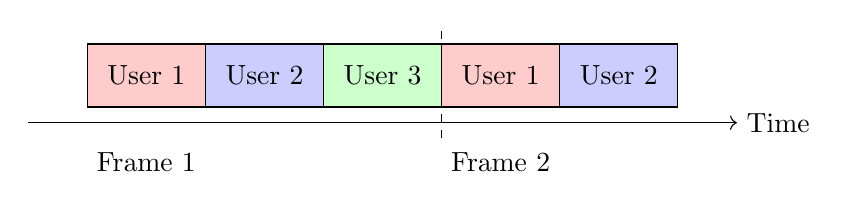
\begin{tikzpicture}[x=1.5cm, y=1cm]
    % Time axis
    \draw[->] (0,0) -- (6,0) node[right] {Time};
    
    % Slots
    \draw[fill=red!20] (0.5,0.2) rectangle (1.5,1) node[midway] {User 1};
    \draw[fill=blue!20] (1.5,0.2) rectangle (2.5,1) node[midway] {User 2};
    \draw[fill=green!20] (2.5,0.2) rectangle (3.5,1) node[midway] {User 3};
    \draw[fill=red!20] (3.5,0.2) rectangle (4.5,1) node[midway] {User 1};
    \draw[fill=blue!20] (4.5,0.2) rectangle (5.5,1) node[midway] {User 2};
    
    \node at (1, -0.5) {Frame 1};
    \node at (4, -0.5) {Frame 2};
    
    \draw[dashed] (3.5, -0.2) -- (3.5, 1.2);
\end{tikzpicture}
\end{answerdiagram}

\begin{answertable}{TDM Characteristics}
\begin{tabulary}{\linewidth}{|L|L|}
\hline
\textbf{Feature} & \textbf{Description} \\
\hline
\textbf{Principle} & Different users allocated different time slots \\
\hline
\textbf{Synchronization} & All devices must be synchronized \\
\hline
\textbf{Efficiency} & Full bandwidth utilization when slots filled \\
\hline
\textbf{Applications} & Digital telephone systems, T1/E1 lines \\
\hline
\end{tabulary}
\end{answertable}

\textbf{TDM Types:}
\begin{itemize}
    \item \textbf{Synchronous TDM}: Fixed time slots regardless of data availability
    \item \textbf{Asynchronous TDM}: Dynamic slot allocation based on demand
    \item \textbf{Statistical TDM}: Slots allocated on statistical basis
\end{itemize}

\textbf{Advantages:}
\begin{itemize}
    \item \textbf{Fair Sharing}: Equal time allocation for all users
    \item \textbf{No Signal Interference}: Time-based separation prevents conflicts
\end{itemize}

\begin{mnemonicbox}
\mnemonic{TDM - Time Divides Medium fairly}
\end{mnemonicbox}
\end{solutionbox}

\questionmarks{3(a OR)}{3}{Explain Amplitude Modulation (AM).}

\begin{solutionbox}
\textbf{Answer:}

\begin{answerdiagram}{AM Signal Concept}
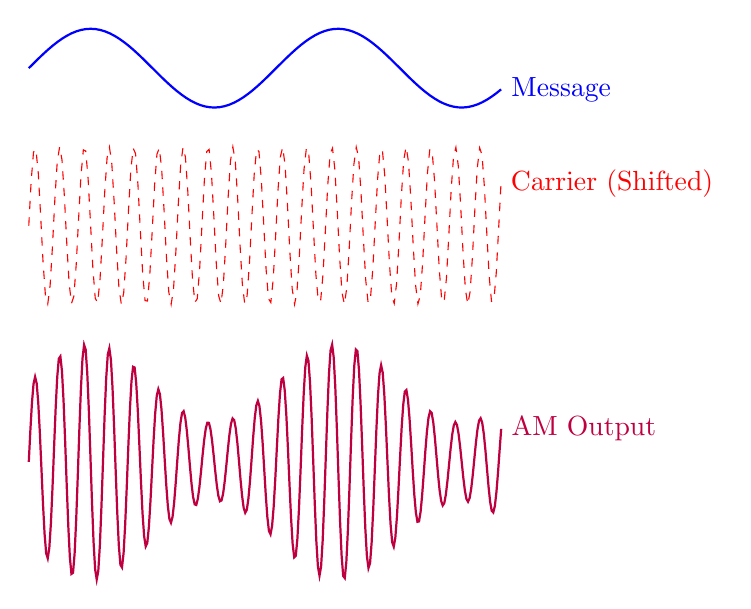
\begin{tikzpicture}
    % Message Signal
    \draw[blue, thick] plot[domain=0:6, samples=100] (\x, {0.5*sin(2*\x r)}) node[right] {Message};
    % Carrier Signal
    \draw[red, dashed] plot[domain=0:6, samples=200] (\x, {sin(20*\x r) - 2}) node[right] {Carrier (Shifted)};
    % AM Signal
    \draw[purple, thick] plot[domain=0:6, samples=300] (\x, {(1 + 0.5*sin(2*\x r)) * sin(20*\x r) - 5}) node[right] {AM Output};
\end{tikzpicture}
\end{answerdiagram}

\begin{answertable}{AM Characteristics}
\begin{tabulary}{\linewidth}{|L|L|}
\hline
\textbf{Parameter} & \textbf{Description} \\
\hline
\textbf{Definition} & Amplitude of carrier varies with message signal \\
\hline
\textbf{Frequency Range} & 535-1605 kHz (AM radio) \\
\hline
\textbf{Bandwidth} & Twice the message signal frequency \\
\hline
\end{tabulary}
\end{answertable}

\begin{itemize}
    \item \textbf{Carrier Wave}: High frequency signal that carries information
    \item \textbf{Modulation Index}: Determines depth of amplitude variation
    \item \textbf{Applications}: AM radio broadcasting, aircraft communication
\end{itemize}

\begin{mnemonicbox}
\mnemonic{AM - Amplitude Modifies with message}
\end{mnemonicbox}
\end{solutionbox}

\questionmarks{3(b OR)}{4}{Describe DNS.}

\begin{solutionbox}
\textbf{Answer:}

\begin{answerdiagram}{DNS Hierarchy}
\begin{tikzpicture}[gtu tree]
    \node [gtu root] {Root (.)}
        child { node [gtu block, fill=yellow!10] {.com} 
            child { node [gtu child] {google.com} 
                child { node [gtu block, fill=orange!10] {mail} }
                child { node [gtu block, fill=orange!10] {www} }
            }
            child { node [gtu child] {microsoft.com} }
        }
        child { node [gtu block, fill=yellow!10] {.org} };
\end{tikzpicture}
\end{answerdiagram}

\begin{answertable}{DNS Components}
\begin{tabulary}{\linewidth}{|L|L|}
\hline
\textbf{Component} & \textbf{Function} \\
\hline
\textbf{Domain Name} & Human-readable web address \\
\hline
\textbf{IP Address} & Numerical address of server \\
\hline
\textbf{DNS Server} & Translates names to IP addresses \\
\hline
\textbf{Records} & Different types (A, MX, CNAME) \\
\hline
\end{tabulary}
\end{answertable}

\begin{itemize}
    \item \textbf{Name Resolution}: Converts domain names to IP addresses
    \item \textbf{Hierarchical Structure}: Root, TLD, second-level domains
    \item \textbf{Distributed Database}: No single point of failure
    \item \textbf{Caching}: Improves performance by storing recent lookups
\end{itemize}

\begin{mnemonicbox}
\mnemonic{DNS - Domain Name System translates addresses}
\end{mnemonicbox}
\end{solutionbox}

\questionmarks{3(c OR)}{7}{Describe following 1. Serial Communication 2. Synchronous Transmission}

\begin{solutionbox}
\textbf{Answer:}

\begin{answerdiagram}{Communication Types}
\begin{tikzpicture}[gtu tree]
    \node [gtu root] {Data Communication}
        child { node [gtu child] {Serial} 
            child { node [gtu block] {Synchronous} }
            child { node [gtu block] {Asynchronous} }
        }
        child { node [gtu child] {Parallel} };
\end{tikzpicture}
\end{answerdiagram}

\begin{answertable}{Communication Comparison}
\begin{tabulary}{\linewidth}{|L|L|L|L|}
\hline
\textbf{Type} & \textbf{Description} & \textbf{Timing} & \textbf{Examples} \\
\hline
\keyword{Serial Communication} & Data bits sent one after another & Slower but reliable & RS-232, USB, Ethernet \\
\hline
\keyword{Synchronous Transmission} & Clock signal synchronizes sender/receiver & Precise timing & HDLC, SDLC \\
\hline
\end{tabulary}
\end{answertable}

\textbf{1. Serial Communication:}
\begin{itemize}
    \item \textbf{Single Wire}: Data transmitted bit by bit over single channel
    \item \textbf{Cost Effective}: Requires fewer wires than parallel
    \item \textbf{Long Distance}: Less susceptible to noise and interference
    \item \textbf{Error Detection}: Built-in mechanisms for data integrity
\end{itemize}

\textbf{2. Synchronous Transmission:}
\begin{itemize}
    \item \textbf{Clock Synchronization}: Separate clock signal or embedded timing
    \item \textbf{Block Transmission}: Data sent in continuous blocks
    \item \textbf{Higher Efficiency}: No start/stop bits needed
    \item \textbf{Complex Hardware}: Requires synchronized clocks
\end{itemize}

\begin{mnemonicbox}
\mnemonic{Serial is Sequential, Synchronous is Simultaneous}
\end{mnemonicbox}
\end{solutionbox}

\questionmarks{4(a)}{3}{Differentiate Mesh and Bus topology.}

\begin{solutionbox}
\textbf{Answer:}

\begin{answertable}{Topology Comparison}
\begin{tabulary}{\linewidth}{|L|L|L|}
\hline
\textbf{Feature} & \textbf{Mesh Topology} & \textbf{Bus Topology} \\
\hline
\textbf{Connection} & Every node connected to every other & All nodes on single cable \\
\hline
\textbf{Fault Tolerance} & Very high & Low (single point of failure) \\
\hline
\textbf{Cost} & Very expensive & Economical \\
\hline
\textbf{Performance} & Excellent & Degrades with more nodes \\
\hline
\end{tabulary}
\end{answertable}

\begin{answerdiagram}{Mesh vs Bus Topology}
\begin{tikzpicture}[node distance=1.5cm]
    % Mesh
    \begin{scope}[shift={(0,0)}]
        \node[gtu state] (A) at (0,2) {A};
        \node[gtu state] (B) at (2,2) {B};
        \node[gtu state] (C) at (0,0) {C};
        \node[gtu state] (D) at (2,0) {D};
        \draw (A)--(B) (A)--(C) (A)--(D) (B)--(C) (B)--(D) (C)--(D);
        \node at (1,-1) {Mesh Topology};
    \end{scope}
    
    % Bus
    \begin{scope}[shift={(4,0.5)}]
       \draw[thick] (0,1) -- (5,1) node[right] {Terminator};
       \draw[thick] (0,1) node[left] {Terminator};
       \node[gtu child] (A) at (0.5,0) {A};
       \node[gtu child] (B) at (2,0) {B};
       \node[gtu child] (C) at (3.5,0) {C};
       \draw (A) -- (0.5,1);
       \draw (B) -- (2,1);
       \draw (C) -- (3.5,1);
       \node at (2.5,-1.5) {Bus Topology};
    \end{scope}
\end{tikzpicture}
\end{answerdiagram}

\begin{itemize}
    \item \textbf{Mesh Advantages}: Redundant paths, high reliability
    \item \textbf{Bus Advantages}: Simple installation, cost-effective
    \item \textbf{Cable Requirements}: Mesh needs n(n-1)/2 connections, Bus needs single cable
\end{itemize}

\begin{mnemonicbox}
\mnemonic{Mesh is Many connections, Bus is Basic single line}
\end{mnemonicbox}
\end{solutionbox}

\questionmarks{4(b)}{4}{Compare FDM and TDM.}

\begin{solutionbox}
\textbf{Answer:}

\begin{answertable}{FDM vs TDM Comparison}
\begin{tabulary}{\linewidth}{|L|L|L|}
\hline
\textbf{Parameter} & \textbf{FDM} & \textbf{TDM} \\
\hline
\textbf{Full Form} & Frequency Division Multiplexing & Time Division Multiplexing \\
\hline
\textbf{Division Basis} & Frequency bands & Time slots \\
\hline
\textbf{Signal Type} & Analog & Digital \\
\hline
\textbf{Crosstalk} & Possible between channels & No crosstalk \\
\hline
\textbf{Synchronization} & Not required & Required \\
\hline
\textbf{Efficiency} & Lower due to guard bands & Higher efficiency \\
\hline
\end{tabulary}
\end{answertable}

\begin{answerdiagram}{Multiplexing Hierarchy}
\begin{tikzpicture}[gtu tree]
    \node [gtu root] {Multiplexing}
        child { node [gtu child] {FDM} 
            child { node [gtu block] {Radio} }
            child { node [gtu block] {Cable TV} }
        }
        child { node [gtu child] {TDM} 
            child { node [gtu block] {Telephony} }
            child { node [gtu block] {Networks} }
        };
\end{tikzpicture}
\end{answerdiagram}

\textbf{FDM Characteristics:}
\begin{itemize}
    \item \textbf{Frequency Separation}: Each signal allocated different frequency band
    \item \textbf{Simultaneous Transmission}: All signals transmitted at same time
    \item \textbf{Guard Bands}: Prevent interference between channels
\end{itemize}

\textbf{TDM Characteristics:}
\begin{itemize}
    \item \textbf{Time Separation}: Each signal allocated different time slot
    \item \textbf{Sequential Transmission}: Signals transmitted one after another
    \item \textbf{Precise Timing}: Requires synchronized clocks
\end{itemize}

\begin{mnemonicbox}
\mnemonic{FDM uses Frequency, TDM uses Time}
\end{mnemonicbox}
\end{solutionbox}

\questionmarks{4(c)}{7}{Draw and illustrate OSI reference model.}

\begin{solutionbox}
\textbf{Answer:}

\begin{answerdiagram}{OSI Reference Model}
\begin{tikzpicture}[node distance=0cm, every node/.style={gtu block, minimum width=6cm, minimum height=0.8cm}]
    \node (app) {7. Application Layer (HTTP, FTP)};
    \node [below=of app] (pres) {6. Presentation Layer (Encryption)};
    \node [below=of pres] (sess) {5. Session Layer (RPC)};
    \node [below=of sess] (trans) {4. Transport Layer (TCP, UDP)};
    \node [below=of trans] (net) {3. Network Layer (IP, Routing)};
    \node [below=of net] (link) {2. Data Link Layer (Ethernet)};
    \node [below=of link] (phy) {1. Physical Layer (Cables, Hubs)};
    
    \draw[->] (app.east) -- ++(1,0) |- (phy.east) node[midway, right] {Data Encapsulation};
    \draw[->] (phy.west) -- ++(-1,0) |- (app.west) node[midway, left] {Data Decapsulation};
\end{tikzpicture}
\end{answerdiagram}

\begin{answertable}{OSI Layer Functions}
\begin{tabulary}{\linewidth}{|C|L|L|L|}
\hline
\textbf{Layer} & \textbf{Name} & \textbf{Function} & \textbf{Examples} \\
\hline
\textbf{7} & Application & User interface & HTTP, FTP, SMTP \\
\hline
\textbf{6} & Presentation & Data formatting & Encryption, Compression \\
\hline
\textbf{5} & Session & Session management & NetBIOS, RPC \\
\hline
\textbf{4} & Transport & End-to-end delivery & TCP, UDP \\
\hline
\textbf{3} & Network & Routing & IP, ICMP \\
\hline
\textbf{2} & Data Link & Frame delivery & Ethernet, PPP \\
\hline
\textbf{1} & Physical & Bit transmission & Cables, Hubs \\
\hline
\end{tabulary}
\end{answertable}

\begin{itemize}
    \item \textbf{Layered Architecture}: Each layer has specific responsibilities
    \item \textbf{Protocol Independence}: Layers can be modified independently
    \item \textbf{Standardization}: Common framework for network communication
    \item \textbf{Encapsulation}: Each layer adds its own header
\end{itemize}

\begin{mnemonicbox}
\mnemonic{All People Seem To Need Data Processing}
\end{mnemonicbox}
\end{solutionbox}

\questionmarks{4(a OR)}{3}{Describe Hub in brief.}

\begin{solutionbox}
\textbf{Answer:}

\begin{answerdiagram}{Network Hub}
\begin{tikzpicture}
    \node[gtu block, minimum width=2cm, minimum height=1cm, fill=gray!20] (hub) {HUB};
    \node[gtu child, above left=of hub] (pc1) {PC1};
    \node[gtu child, above right=of hub] (pc2) {PC2};
    \node[gtu child, below=of hub] (pc3) {PC3};
    \draw (hub) -- (pc1);
    \draw (hub) -- (pc2);
    \draw (hub) -- (pc3);
\end{tikzpicture}
\end{answerdiagram}

\begin{answertable}{Hub Characteristics}
\begin{tabulary}{\linewidth}{|L|L|}
\hline
\textbf{Feature} & \textbf{Description} \\
\hline
\textbf{Function} & Central connection point for devices \\
\hline
\textbf{Type} & Physical layer device (Layer 1) \\
\hline
\textbf{Data Handling} & Broadcasts to all connected devices \\
\hline
\textbf{Collision Domain} & All ports share same collision domain \\
\hline
\end{tabulary}
\end{answertable}

\begin{itemize}
    \item \textbf{Shared Bandwidth}: All connected devices share total bandwidth
    \item \textbf{Half-Duplex}: Cannot send and receive simultaneously
    \item \textbf{Security Issues}: All devices receive all transmitted data
    \item \textbf{Obsolete Technology}: Replaced by switches in modern networks
\end{itemize}

\begin{mnemonicbox}
\mnemonic{Hub is Half-duplex, shares Bandwidth}
\end{mnemonicbox}
\end{solutionbox}

\questionmarks{4(b OR)}{4}{Compare STP and UTP.}

\begin{solutionbox}
\textbf{Answer:}

\begin{answertable}{STP vs UTP Cable Comparison}
\begin{tabulary}{\linewidth}{|L|L|L|}
\hline
\textbf{Feature} & \textbf{STP (Shielded)} & \textbf{UTP (Unshielded)} \\
\hline
\textbf{Shielding} & Metal foil/braid protection & No shielding \\
\hline
\textbf{Cost} & More expensive & Less expensive \\
\hline
\textbf{Installation} & Complex due to grounding & Simple installation \\
\hline
\textbf{EMI Resistance} & Excellent protection & Moderate protection \\
\hline
\textbf{Applications} & Industrial environments & Office environments \\
\hline
\end{tabulary}
\end{answertable}

\begin{answerdiagram}{Cable Structure}
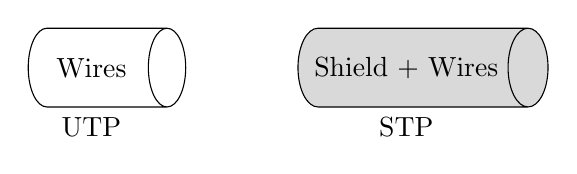
\begin{tikzpicture}
    % UTP
    \node[draw, cylinder, shape border rotate=0, minimum height=2cm, minimum width=1cm, label=below:UTP] (utp) at (0,0) {Wires};
    
    % STP
    \node[draw, cylinder, shape border rotate=0, minimum height=2cm, minimum width=1cm, fill=gray!30, label=below:STP] (stp) at (4,0) {Shield + Wires};
\end{tikzpicture}
\end{answerdiagram}

\begin{itemize}
    \item \textbf{STP Advantages}: Better noise immunity, higher data rates, secure transmission
    \item \textbf{UTP Advantages}: Cost effective, easy installation, flexible
\end{itemize}

\begin{mnemonicbox}
\mnemonic{STP is Shielded but Pricey, UTP is Unshielded but Popular}
\end{mnemonicbox}
\end{solutionbox}

\questionmarks{4(c OR)}{7}{Distinguish LAN, MAN, WAN.}

\begin{solutionbox}
\textbf{Answer:}

\begin{answerdiagram}{Network Types Hierarchy}
\begin{tikzpicture}[gtu tree]
    \node [gtu root] {Computer Networks}
        child { node [gtu child] {LAN} 
            child { node [gtu block] {Campus} }
        }
        child { node [gtu child] {MAN} 
            child { node [gtu block] {City} }
        }
        child { node [gtu child] {WAN} 
            child { node [gtu block] {Global} }
        };
\end{tikzpicture}
\end{answerdiagram}

\begin{answertable}{Network Type Comparison}
\begin{tabulary}{\linewidth}{|L|L|L|L|}
\hline
\textbf{Parameter} & \textbf{LAN} & \textbf{MAN} & \textbf{WAN} \\
\hline
\textbf{Coverage} & Building/Campus & City/Metropolitan & Country/Global \\
\hline
\textbf{Speed} & High (1 Gbps+) & Medium & Lower/Variable \\
\hline
\textbf{Cost} & Low & Medium & High \\
\hline
\textbf{Ownership} & Private & Private/Public & Public/Leased \\
\hline
\textbf{Technology} & Ethernet, Wi-Fi & Fiber, WiMAX & Satellite, Leased \\
\hline
\end{tabulary}
\end{answertable}

\begin{itemize}
    \item \textbf{LAN (Local Area Network)}: High speed, low cost, private ownership
    \item \textbf{MAN (Metropolitan Area Network)}: City-wide, medium speed, mixed ownership
    \item \textbf{WAN (Wide Area Network)}: Global coverage, public infrastructure, variable speed
\end{itemize}

\begin{mnemonicbox}
\mnemonic{LAN is Local, MAN is Metropolitan, WAN is Wide}
\end{mnemonicbox}
\end{solutionbox}

\questionmarks{5(a)}{3}{Explain Denial of Service Attack.}

\begin{solutionbox}
\textbf{Answer:}

\begin{answerdiagram}{DoS Attack}
\begin{tikzpicture}
    \node[gtu block, fill=red!10] (attacker) {Attacker};
    \node[gtu block, right=4cm of attacker] (target) {Target Server};
    
    \draw[->, thick, red] (attacker) -- (target) node[midway, above] {Request 1};
    \draw[->, thick, red] (attacker.north) to[bend left=20] node[midway, above] {Request 2} (target.north);
    \draw[->, thick, red] (attacker.south) to[bend right=20] node[midway, below] {Request 3...N} (target.south);
    
    \node[below=0.5cm of target, text width=3cm, align=center] {Overwhelmed};
\end{tikzpicture}
\end{answerdiagram}

\begin{itemize}
    \item \textbf{Definition}: Attack where legitimate users are unable to access information systems or devices
    \item \textbf{Mechanism}: Flooding the target with excess requests to overload system resources
    \item \textbf{Impact}: Service downtime, financial loss, reputation damage
\end{itemize}

\end{solutionbox}


\questionmarks{5(b)}{4}{i) Classify data transmission ii) Write down use of Terminator in Bus Topology.}

\begin{solutionbox}
\textbf{Answer:}

\textbf{i) Data Transmission Classification:}

\begin{answerdiagram}{Data Transmission Types}
\begin{tikzpicture}[gtu tree]
    \node [gtu root] {Data Transmission}
        child { node [gtu child] {Direction} 
            child { node [gtu block] {Simplex} }
            child { node [gtu block] {Half-Duplex} }
            child { node [gtu block] {Full-Duplex} }
        }
        child { node [gtu child] {Timing} 
            child { node [gtu block] {Synchronous} }
            child { node [gtu block] {Asynchronous} }
        }
        child { node [gtu child] {Mode} 
            child { node [gtu block] {Serial} }
            child { node [gtu block] {Parallel} }
        };
\end{tikzpicture}
\end{answerdiagram}

\textbf{ii) Terminator in Bus Topology:}

\begin{answertable}{Terminator Functions}
\begin{tabulary}{\linewidth}{|L|L|}
\hline
\textbf{Function} & \textbf{Description} \\
\hline
\textbf{Signal Absorption} & Prevents signal reflection \\
\hline
\textbf{Impedance Matching} & Matches cable impedance \\
\hline
\textbf{Network Integrity} & Maintains signal quality \\
\hline
\end{tabulary}
\end{answertable}

\begin{itemize}
    \item \textbf{Prevention of Reflection}: Stops signals from bouncing back
    \item \textbf{Signal Quality}: Maintains clean signal transmission
    \item \textbf{Required at Both Ends}: Bus topology needs terminators at both cable ends
    \item \textbf{Resistance Value}: Usually 50 ohms for Ethernet networks
\end{itemize}

\begin{mnemonicbox}
\mnemonic{Terminator Stops signal Travel}
\end{mnemonicbox}
\end{solutionbox}

\questionmarks{5(c)}{7}{Describe CIA triad.}

\begin{solutionbox}
\textbf{Answer:}

\begin{answerdiagram}{CIA Triad}
\begin{tikzpicture}[gtu tree]
    \node [gtu root] {CIA Triad}
        child { node [gtu child] {Confidentiality} 
            child { node [gtu block] {Encryption} }
            child { node [gtu block] {Access Control} }
        }
        child { node [gtu child] {Integrity} 
            child { node [gtu block] {Hash Functions} }
            child { node [gtu block] {Digital Signatures} }
        }
        child { node [gtu child] {Availability} 
            child { node [gtu block] {Redundancy} }
            child { node [gtu block] {Backup Systems} }
        };
\end{tikzpicture}
\end{answerdiagram}

\begin{answertable}{CIA Triad Components}
\begin{tabulary}{\linewidth}{|L|L|L|L|}
\hline
\textbf{Component} & \textbf{Definition} & \textbf{Implementation} & \textbf{Threats} \\
\hline
\textbf{Confidentiality} & Information secrecy & Encryption, Access control & Unauthorized disclosure \\
\hline
\textbf{Integrity} & Data accuracy and completeness & Hash functions, Digital signatures & Data modification \\
\hline
\textbf{Availability} & Information accessibility & Redundancy, Backup systems & Service disruption \\
\hline
\end{tabulary}
\end{answertable}

\textbf{Confidentiality:}
\begin{itemize}
    \item \textbf{Data Protection}: Only authorized users can access information
    \item \textbf{Privacy Measures}: Encryption, authentication, access controls
    \item \textbf{Examples}: Password protection, file permissions
\end{itemize}

\textbf{Integrity:}
\begin{itemize}
    \item \textbf{Data Accuracy}: Information remains unaltered during transmission/storage
    \item \textbf{Verification Methods}: Checksums, digital signatures, version control
    \item \textbf{Examples}: Hash functions, database constraints
\end{itemize}

\textbf{Availability:}
\begin{itemize}
    \item \textbf{System Accessibility}: Information and services available when needed
    \item \textbf{Reliability Measures}: Redundancy, fault tolerance, disaster recovery
    \item \textbf{Examples}: Load balancing, backup systems, UPS
\end{itemize}

\begin{mnemonicbox}
\mnemonic{CIA protects - Confidentiality, Integrity, Availability}
\end{mnemonicbox}
\end{solutionbox}

\questionmarks{5(a OR)}{3}{Define: 1. Cryptography 2. Decryption}

\begin{solutionbox}
\textbf{Answer:}

\begin{answertable}{Definition Table}
\begin{tabulary}{\linewidth}{|L|L|L|}
\hline
\textbf{Term} & \textbf{Definition} & \textbf{Purpose} \\
\hline
\keyword{Cryptography} & Science of securing information through encoding & Protect data confidentiality \\
\hline
\keyword{Decryption} & Process of converting encrypted data back to original & Retrieve original information \\
\hline
\end{tabulary}
\end{answertable}

\begin{itemize}
    \item \textbf{Cryptography}: Uses mathematical algorithms to transform readable data into unreadable format
    \item \textbf{Decryption}: Reverse process using keys to restore original data
    \item \textbf{Key-based Security}: Both processes rely on cryptographic keys
\end{itemize}

\begin{mnemonicbox}
\mnemonic{Crypto Conceals, Decryption Discloses}
\end{mnemonicbox}
\end{solutionbox}

\questionmarks{5(b OR)}{4}{i) State reason why wires are twisted in twisted pair cables. ii) Identify OSI layer for: 1. Router 2. Bridge}

\begin{solutionbox}
\textbf{Answer:}

\textbf{i) Twisted Pair Cable Design:}

\begin{answertable}{Wire Twisting Benefits}
\begin{tabulary}{\linewidth}{|L|L|}
\hline
\textbf{Benefit} & \textbf{Description} \\
\hline
\textbf{Noise Reduction} & Cancels electromagnetic interference \\
\hline
\textbf{Crosstalk Prevention} & Reduces signal interference between pairs \\
\hline
\textbf{Signal Quality} & Maintains better signal integrity \\
\hline
\end{tabulary}
\end{answertable}

\textbf{ii) OSI Layer Identification:}

\begin{answertable}{Network Devices and OSI Layers}
\begin{tabulary}{\linewidth}{|L|L|L|}
\hline
\textbf{Device} & \textbf{OSI Layer} & \textbf{Function} \\
\hline
\textbf{Router} & Layer 3 (Network) & Routing between different networks \\
\hline
\textbf{Bridge} & Layer 2 (Data Link) & Connecting network segments \\
\hline
\end{tabulary}
\end{answertable}

\begin{itemize}
    \item \textbf{Wire Twisting}: Each twist cancels out electromagnetic interference from adjacent wire
    \item \textbf{Interference Cancellation}: Noise affects both wires equally but in opposite directions
    \item \textbf{Router Function}: Makes routing decisions based on IP addresses
    \item \textbf{Bridge Function}: Forwards frames based on MAC addresses
\end{itemize}

\begin{mnemonicbox}
\mnemonic{Twisted wires Reduce interference, Router at layer 3, Bridge at layer 2}
\end{mnemonicbox}
\end{solutionbox}

\questionmarks{5(c OR)}{7}{Define Cyber Attack and explain various cyber-attacks in brief}

\begin{solutionbox}
\textbf{Answer:}

\textbf{Cyber Attack Definition:}
Cyber attack is a deliberate attempt to compromise computer systems, networks, or digital devices to steal, alter, or destroy data.

\begin{answerdiagram}{Cyber Attack Types}
\begin{tikzpicture}[gtu tree]
    \node [gtu root] {Cyber Attacks}
        child { node [gtu child] {Malware} 
            child { node [gtu block, fill=red!10] {Virus, Worm, Trojan} }
        }
        child { node [gtu child] {Phishing} 
            child { node [gtu block, fill=orange!10] {Email, Website} }
        }
        child { node [gtu child] {DoS/DDoS} 
            child { node [gtu block, fill=yellow!10] {Traffic Flooding} }
        }
        child { node [gtu child] {Man-in-Middle} 
            child { node [gtu block, fill=blue!10] {Eavesdropping} }
        }
        child { node [gtu child] {SQL Injection} 
            child { node [gtu block, fill=green!10] {Database Attack} }
        };
\end{tikzpicture}
\end{answerdiagram}

\begin{answertable}{Cyber Attack Types}
\begin{tabulary}{\linewidth}{|L|L|L|L|}
\hline
\textbf{Attack Type} & \textbf{Description} & \textbf{Impact} & \textbf{Prevention} \\
\hline
\textbf{Malware} & Malicious software (virus, worm, trojan) & System corruption, data theft & Antivirus, updates \\
\hline
\textbf{Phishing} & Fraudulent emails/websites to steal credentials & Identity theft, financial loss & User awareness, email filters \\
\hline
\textbf{DoS/DDoS} & Overwhelming target with traffic & Service unavailability & Firewalls, load balancers \\
\hline
\textbf{Man-in-Middle} & Intercepting communication between parties & Data eavesdropping & Encryption, secure protocols \\
\hline
\textbf{SQL Injection} & Malicious code inserted into database queries & Database compromise & Input validation, parameterized queries \\
\hline
\end{tabulary}
\end{answertable}

\textbf{Malware Attacks:}
\begin{itemize}
    \item \textbf{Virus}: Self-replicating code that attaches to files
    \item \textbf{Worm}: Standalone malware that spreads across networks
    \item \textbf{Trojan}: Disguised malware that appears legitimate
\end{itemize}

\textbf{Social Engineering:}
\begin{itemize}
    \item \textbf{Phishing}: Fake emails requesting sensitive information
    \item \textbf{Spear Phishing}: Targeted attacks on specific individuals
    \item \textbf{Baiting}: Using attractive offers to deliver malware
\end{itemize}

\textbf{Network Attacks:}
\begin{itemize}
    \item \textbf{Packet Sniffing}: Capturing network traffic for analysis
    \item \textbf{Session Hijacking}: Taking over user sessions
    \item \textbf{Password Attacks}: Brute force, dictionary attacks
\end{itemize}

\begin{mnemonicbox}
\mnemonic{MPDMS - Malware, Phishing, DoS, Man-in-middle, SQL injection}
\end{mnemonicbox}
\end{solutionbox}

\end{document}
